\documentclass[conference]{IEEEtran}

\usepackage{amsmath}
\usepackage{booktabs}
\usepackage{graphicx}
\usepackage{microtype}
\usepackage{tabularx}
\usepackage{array}
\usepackage{xurl}
\usepackage{cite}
\usepackage{balance}

\newcolumntype{Y}{>{\raggedright\arraybackslash}X}
\newcommand{\pct}{\%}

\title{Stated or Revealed Risk? Out-of-Time Prediction of Retail Investor Trading after Extreme Negative Returns}

\author{\IEEEauthorblockN{Dongha Park}
\IEEEauthorblockA{Independent Researcher\\
Republic of Korea}}

\begin{document}
\maketitle

\begin{abstract}
Financial institutions use questionnaire-based risk profiles for suitability, but the value of those profiles for predicting near-term trading during losses is uncertain. Using the public FAR-Trans dataset, this study compares stated customer profiles with behavior revealed in prior transactions across repeated account-level exposures to security-specific extreme negative returns. Descriptive analysis, clustered regressions, and chronological machine-learning validation show that stated risk categories do not consistently order short-horizon responses and add little stable predictive value once event, position, and behavioral information are considered. General transaction history is more consistently informative, while the incremental value of earlier responses to similar events varies with event-screening choices. The results do not challenge the suitability role of risk profiles; they indicate that suitability classification and short-horizon behavioral prediction are distinct measurement tasks.
\end{abstract}

\begin{IEEEkeywords}
retail investors, risk tolerance, MiFID, revealed behavior, extreme returns, behavioral finance, out-of-time validation
\end{IEEEkeywords}

\section{Introduction}
Under the European suitability framework, an investment firm providing advice or portfolio management must obtain information about a client's knowledge and experience, financial situation, ability to bear losses, investment objectives, and risk tolerance \cite{eurlex2014mifid,esma2023suitability}. Institutions often summarize part of this information in broad categories such as Conservative, Income, Balanced, or Aggressive. These categories support product eligibility, portfolio construction, and communication, but they are not direct labels for every behavior that may occur during market stress.

This paper asks whether a stated customer profile improves prediction of trading during the five trading days after a security-specific extreme negative return, beyond event characteristics, position information, and the customer's earlier observed behavior. A willingness to hold risk over a long horizon need not imply immediate trading after a loss, which may also reflect attention, liquidity needs, beliefs about reversal, and the affected position. The distinction is relevant to securities firms and bank wealth-management units that use customer analytics for monitoring, segmentation, service-capacity planning, or model review.

The analysis uses FAR-Trans, a public dataset containing anonymized profiles, transactions, asset information, and daily prices from a large European financial institution \cite{sanzcruzado2024fartrans}. We construct repeated customer--security exposures to extreme negative-return events and separate description, adjusted association, and chronological prediction. Models are trained on 2019--2020 observations, tuned and calibrated on 2021 observations, and evaluated once on a 2022 holdout.

The paper contributes by evaluating suitability categories against repeated realized loss-event responses, isolating the incremental value of stated and revealed information, and validating the comparison chronologically under alternative event screens. The results favor observed transaction history for this specific behavioral target, without treating that finding as a rejection of suitability classification.

\section{Related Literature}
\subsection{Stated Risk and Revealed Investment Behavior}
Questionnaire measures of risk tolerance are related to portfolio choice, but they do not always coincide with observed risk taking. Prior work links risk-tolerance scores to portfolio risk \cite{corter2006risk}, examines which questionnaire items explain allocation preferences and investment changes \cite{guillemette2012questions}, and compares elicited risk with risk revealed in client portfolios \cite{thompson2022gap}.

Studies combining surveys with brokerage records are especially relevant. Hoffmann, Post, and Pennings relate time-varying perceptions and risk tolerance to account behavior during the financial crisis \cite{hoffmann2013perceptions,hoffmann2015trading}. Merkle and Weber examine whether stated market expectations are reflected in investment behavior \cite{merkle2014money}. Bellofatto, D'Hondt, and De Winne connect MiFID information to retail trading and portfolio behavior \cite{bellofatto2018literacy}, while Klocke and Pelster use MiFID II questionnaire information to study retail short sellers \cite{klocke2026short}. Brooks and Williams show that conventional risk-tolerance measures do not cleanly distinguish stated intentions to sell or hold under realistic loss scenarios \cite{brooks2022crunch}. The present study differs by using realized transactions, repeated security-specific events, and an out-of-time prediction design.

\subsection{Trading after Salient Returns}
Extreme returns can attract attention and alter retail trading. Attention-grabbing events affect individual-investor buying \cite{barber2008glitters}, while loss realization may also reflect the disposition effect or beliefs about mean reversion \cite{odean1998losses}. These mechanisms imply no single response to a decline: an investor may purchase, sell, or remain inactive.

Prior event-based studies identify large losses using fixed one-day declines, security-specific standardized tails, or rolling empirical tails \cite{cox1994declines,guo2024extreme,cardozo2026tail}. The rule used here is a study-specific hybrid that combines an economically material raw loss with a security-specific empirical tail of market-adjusted abnormal returns. The abnormal-return construction follows standard market-model event-study logic \cite{mackinlay1997event}. Because the data do not identify an exogenous news shock and lack a complete corporate-action history, the neutral term \emph{extreme negative-return event} is used.

FAR-Trans was introduced as a benchmark for predicting which assets a customer may purchase next \cite{sanzcruzado2024fartrans}. This paper instead studies whether a current holder trades after an extreme loss and whether stated profile information adds predictive value after prior behavior is observed. The contribution lies in combining repeated account-level events, stated-versus-revealed information, and chronological validation; no universal priority claim is made.

\section{Data and Empirical Design}
\subsection{FAR-Trans and Customer Eligibility}
FAR-Trans contains customer profiles, asset metadata, market information, daily closing prices, and transactions \cite{sanzcruzado2024fartrans}. Customer profiles may appear more than once as information is updated. The available risk field includes observed categories, algorithmically predicted categories, and missing values. The primary sample keeps Mass and Premium retail clients whose latest eligible profile records contain an observed Conservative, Income, Balanced, or Aggressive category. For every prediction observation, the questionnaire date must be on or before the return event. Algorithmically predicted risk labels are excluded because they are derived from other customer information and would blur the distinction between stated and revealed information.

The security universe consists of stocks traded under the XATH market code. A security must have at least 500 valid daily closing prices and nonzero returns on at least 30\pct{} of observed days. These requirements leave 134 stocks with enough history for a rolling tail estimate.

FAR-Trans includes reconstructed purchases for holdings that predate the transaction window. Such records have negative transaction identifiers. Because their original purchase dates and cost bases are not observed, every customer--security pair containing a reconstructed purchase is excluded. Holdings are accumulated only from observed nonnegative transactions. A customer is exposed to an event only when strictly positive units are held immediately before the event date.

\begin{table}[t]
\caption{Construction of the Primary Analysis Sample}
\label{tab:sample}
\centering
\footnotesize
\begin{tabular}{lr}
\toprule
Sample stage & Count \\
\midrule
Unique customers in the source data & 29,090 \\
Mass or Premium clients with observed risk & 20,412 \\
Price-eligible XATH stocks & 134 \\
Customers in the final analysis sample & 5,492 \\
Extreme-return events represented & 552 \\
Customer--security--event exposures & 35,424 \\
Trades within five trading days & 2,482 \\
Purchases within five trading days & 1,420 \\
Sales within five trading days & 1,062 \\
\bottomrule
\end{tabular}
\end{table}

\subsection{Extreme Negative-Return Events}
For each date, the primary market-return proxy is the cross-sectional median return among eligible XATH stocks. The median can be constructed entirely from the licensed dataset and reduces the influence of a small number of extreme observations. For security $i$ and date $t$, a rolling market model is estimated over trading days $t-260$ through $t-11$:
\begin{equation}
 r_{i,s}=\alpha_{i,t}+\beta_{i,t}r_{m,s}+\varepsilon_{i,s},
 \qquad s\in[t-260,t-11].
\end{equation}
At least 200 observations are required. The abnormal return on the candidate event date is
\begin{equation}
 AR_{i,t}=r_{i,t}-\left(\widehat{\alpha}_{i,t}+\widehat{\beta}_{i,t}r_{m,t}\right).
\end{equation}
An event is retained when the raw daily return is no greater than $-5\pct{}$ and the abnormal return is at or below the security's empirical first percentile estimated from the prior rolling window. This exact combined rule is an operational choice of the present study rather than a threshold copied from a single prior paper. The raw threshold imposes economic materiality, while the security-specific tail condition adapts the screen to differences in historical volatility. For a given security, candidate events within 20 trading days of an earlier retained event are removed to limit overlapping episodes. A broad-market indicator equals one when at least 5\pct{} of eligible securities satisfy the event rule on the same date.

\subsection{Response Labels}
FAR-Trans provides transaction dates but not intraday order times, so event-day transactions are excluded because their ordering relative to the closing-price movement is unknown. The primary response window begins on the next trading day and ends after five trading days. The first observed transaction in the affected security defines the response as purchase or sale; otherwise the response is no action. Alternative windows of one, ten, and twenty trading days are used for robustness.

The primary prediction task is action versus no action. A secondary model predicts sale versus purchase conditional on action, avoiding a single multiclass formulation dominated by inactivity.

\subsection{Information Available before Each Event}
All predictors are dated strictly before the event. Table~\ref{tab:features} groups them into event and position information, stated customer profiles, general historical trading behavior, and earlier responses to extreme negative returns.

The final group summarizes earlier responses to extreme negative returns. For customer $j$, the smoothed historical action rate before time $t$ is
\begin{equation}
 \frac{A_{j,t^-}+1}{E_{j,t^-}+2},
\end{equation}
where $E_{j,t^-}$ is the number of earlier eligible event exposures and $A_{j,t^-}$ is the number followed by an action. A corresponding smoothed sale rate is formed among earlier actions. Events on the same date are treated as contemporaneous, and no response from the current or a later event contributes to the predictors.

\begin{table*}[t]
\caption{Information Sets Used in Inference and Prediction}
\label{tab:features}
\centering
\footnotesize
\begin{tabularx}{\textwidth}{p{0.23\textwidth}Y}
\toprule
Information set & Information included \\
\midrule
Event and position information & Raw security return, market-adjusted abnormal return, market return, broad-market indicator, sector, units held, estimated position value, number of earlier trades in the affected security, and time since the customer's most recent trade in that security. \\
Stated customer profile & Observed risk category, investment-capacity category, Mass or Premium customer type, and number of days elapsed since the most recent eligible questionnaire. \\
Historical trading behavior & Cumulative number of earlier transactions, historical purchase share, stock-transaction share, internet-channel share, average transaction value, transactions during the preceding 90 days, number of distinct assets traded, and time since any transaction. \\
Earlier extreme-event response & Number of earlier eligible extreme-return exposures, smoothed historical probability of taking action after those events, and smoothed historical probability of selling conditional on action. \\
\bottomrule
\end{tabularx}
\end{table*}

\subsection{Inference, Prediction, and Uncertainty}
Binomial generalized linear models are estimated for action versus no action and, among actors, sale versus purchase. Numeric predictors are standardized, and standard errors are clustered simultaneously by customer and date--security event to account for both forms of dependence \cite{cameron2011multiway}. Coefficients are interpreted as adjusted associations rather than causal effects.

CatBoost classifiers are used for prediction because the data combine numeric and categorical information \cite{prokhorenkova2018catboost}. Observations from 2019 and 2020 form the training set, 2021 observations are used for early stopping and sigmoid calibration, and 2022 observations are evaluated once as an out-of-time holdout \cite{platt1999probabilistic}. Five nested information sets compare event and position information, customer profiles, general trading history, and earlier extreme-event responses.

Because actions occur in only 7.01\pct{} of primary exposures, precision--recall area is the primary ranking metric; receiver-operating-characteristic area, Brier score, log loss, calibration, and concentration among the highest-scored observations are supplementary measures \cite{saito2015precision}. Differences between models are evaluated with 300 event-block bootstrap draws that resample complete date--security events \cite{efron1993bootstrap}. The accompanying artifact package contains the construction code, executed notebooks, derived analysis data, result tables, validation records, and figure-generation scripts.

\section{Results}
\subsection{Observed Responses by Stated Risk Category}
Table~\ref{tab:risk} reports five-day responses. Action rates rise from Conservative through Balanced customers and then fall for Aggressive customers, so the categories do not form a monotonic behavioral ranking. Purchase and sale rates also differ across categories, but these unadjusted differences may reflect position size, activity, and event composition.

\begin{table}[t]
\caption{Five-Day Responses by Observed Risk Category}
\label{tab:risk}
\centering
\footnotesize
\begin{tabular}{lrrrr}
\toprule
Risk category & Exposures & Action & Purchase & Sale \\
\midrule
Conservative & 1,243 & 5.07\pct{} & 2.57\pct{} & 2.49\pct{} \\
Income & 11,965 & 6.77\pct{} & 3.89\pct{} & 2.88\pct{} \\
Balanced & 16,124 & 7.42\pct{} & 4.20\pct{} & 3.22\pct{} \\
Aggressive & 6,092 & 6.76\pct{} & 4.02\pct{} & 2.74\pct{} \\
\bottomrule
\end{tabular}
\end{table}

\begin{figure}[t]
\centering
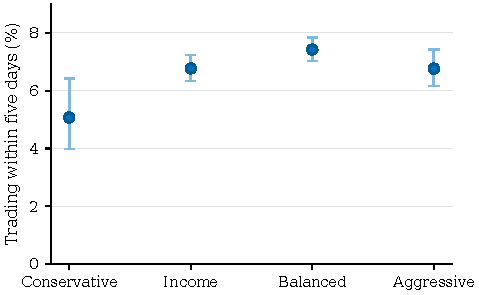
\includegraphics[width=\columnwidth]{figures/fig1_response_by_risk.pdf}
\caption{Observed five-day action rates and Wilson 95\pct{} intervals. The categories do not form a monotonic behavioral ranking.}
\label{fig:risk}
\end{figure}

\subsection{Adjusted Associations}
After event, position, profile, and behavioral controls are included, the risk-category estimates remain imprecise: all confidence intervals for action include one. In contrast, cumulative prior transaction count, recent transaction activity, and the customer's smoothed historical action rate after earlier extreme returns are positively associated with action. Larger position value is also positively associated with action, while a longer time since the last trade in the affected security is negatively associated with action. Figure~\ref{fig:odds} displays selected estimates.

Conditional on action, risk-category estimates for selling rather than purchasing are also imprecise. The customer's smoothed prior sale rate is more informative, with an adjusted odds ratio of 1.24 per standard deviation and a 95\pct{} confidence interval of 1.12--1.38. These associations describe persistence in observed response type and are not causal estimates.

\begin{figure}[t]
\centering
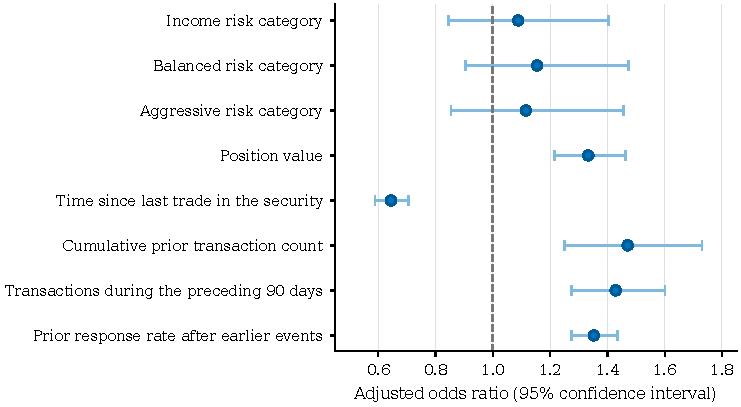
\includegraphics[width=\columnwidth]{figures/fig2_selected_odds_ratios.pdf}
\caption{Selected adjusted associations with any action. Numeric predictors are standardized; risk-category estimates use Conservative customers as the reference. Standard errors are clustered by customer and event.}
\label{fig:odds}
\end{figure}

\subsection{Out-of-Time Prediction}
The chronological split contains 10,135 training observations from 2019--2020, 7,997 validation observations from 2021, and 17,292 test observations from 2022. The action rate falls sharply in the test period, as shown in Fig.~\ref{fig:year}; a random split would mix these regimes and would not represent the intended deployment question.

\begin{figure}[t]
\centering
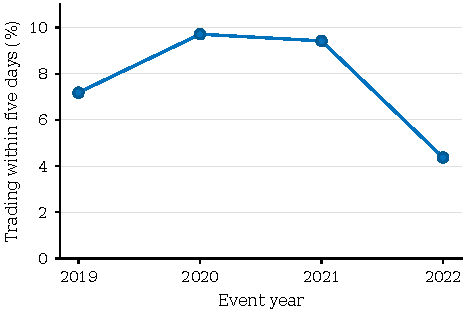
\includegraphics[width=\columnwidth]{figures/fig3_response_by_year.pdf}
\caption{Five-day action rates by event year. The marked decline in 2022 motivates chronological rather than random validation.}
\label{fig:year}
\end{figure}

Table~\ref{tab:prediction} reports the 2022 results. Adding the customer-profile bundle to event and position information does not improve precision--recall ranking. Historical trading behavior provides a modest gain, and the full information set including earlier extreme-event responses performs best in the primary sample. Figure~\ref{fig:prediction} reports bootstrap uncertainty for the incremental comparisons rather than repeating the absolute scores.

\begin{table*}[t]
\caption{Prediction of Any Trading Action in the 2022 Out-of-Time Holdout}
\label{tab:prediction}
\centering
\footnotesize
\begin{tabularx}{\textwidth}{Yrrrr}
\toprule
Information available to the model & Precision--recall area & Receiver-operating-characteristic area & Brier score & Log loss \\
\midrule
Event and position information & 0.245 & 0.826 & 0.0375 & 0.1513 \\
Event, position, and customer profile information & 0.243 & 0.828 & 0.0375 & 0.1510 \\
Event, position, and historical trading behavior & 0.253 & 0.831 & 0.0370 & 0.1459 \\
Event, position, profile, and historical trading behavior & 0.256 & 0.826 & 0.0369 & 0.1464 \\
Full information including earlier responses to extreme returns & 0.286 & 0.840 & 0.0363 & 0.1421 \\
\bottomrule
\end{tabularx}
\end{table*}

\begin{figure}[t]
\centering
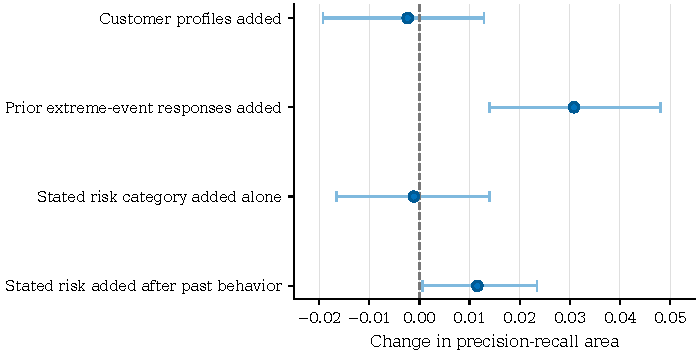
\includegraphics[width=\columnwidth]{figures/fig4_action_model_performance.pdf}
\caption{Event-block bootstrap estimates of incremental changes in precision--recall area. Points show mean changes and horizontal lines show 95\pct{} bootstrap intervals. Each comparison is measured relative to the corresponding baseline model described in the text.}
\label{fig:prediction}
\end{figure}

Event-block bootstrap intervals reinforce the distinction between profiles and revealed behavior. Adding the customer-profile bundle to the event-and-position model yields a mean precision--recall change of $-0.0023$ with an interval spanning zero. Adding earlier extreme-event responses to the profile-and-behavior model yields a positive mean change of 0.0308 in the primary sample. The risk category provides at most a small conditional ranking increment after historical behavior is already included, without a corresponding improvement in receiver-operating-characteristic area.

Among the top 5\pct{} of test observations, the full model captures 36.6\pct{} of actions with 31.9\pct{} precision, compared with 34.6\pct{} recall and 30.2\pct{} precision for the event-and-position model. The gain may support prioritization, but not automatic client intervention without institution-specific validation.

Calibration by probability decile is reasonable in the holdout. Conditional on trading, the full information model attains only modest discrimination between sales and purchases, supporting a separate second stage rather than treating purchase, sale, and no action as balanced outcomes.

\section{Robustness and Validation}
\begin{figure*}[t]
\centering
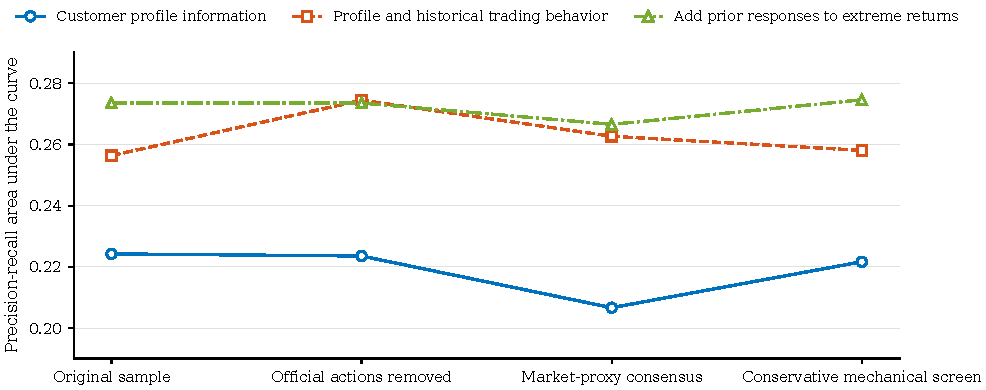
\includegraphics[width=0.96\textwidth]{figures/fig5_external_validation.pdf}
\caption{Independent LightGBM robustness reruns across event-screening specifications. General historical trading behavior improves ranking in every sample; the additional gain from earlier extreme-event responses varies with the screen.}
\label{fig:external}
\end{figure*}

\subsection{Alternative Windows and Event Definitions}
The non-monotonic ordering is not specific to the five-day horizon. Balanced customers remain more active than Aggressive customers and Conservative customers remain least active under one-, ten-, and twenty-day windows, a three-standard-deviation event rule, and an idiosyncratic-only event sample.

Broad-market events show a different, exploratory pattern: action rates rise from 4.52\pct{} for Conservative customers to 10.40\pct{} for Aggressive customers. This smaller subsample suggests that broad risk categories may be more behaviorally visible during common market stress than during firm-specific declines.

\subsection{Market Benchmark and Corporate Actions}
The official benchmark relevant to the sample is the ATHEX Composite Share Price Index, and the corresponding Bank of Greece historical source was verified \cite{athex2026composite,bankofgreece2026indices}. Because the binary daily workbook could not be retrieved in the analysis runtime, the primary event construction was instead repeated with the cross-sectional median, equal-weight mean, 10\pct{} trimmed mean, and 2\pct{} winsorized mean. A consensus sample retains events identified by at least three of the four internal proxies.

Official Athens Exchange materials identify four high-confidence corporate-action overlaps with the event sample: three ATTICA BANK events and one PIRAEUS capital-restructuring event \cite{athex2026actions}. A conservative screen additionally removes non-broad declines of at least 20\pct{}, returns near round $-20\pct{}$ or $-30\pct{}$ bands, and events following long price gaps. These screens test whether the main comparison is driven by mechanical price movements rather than ordinary market losses.

\subsection{Independent Model-Family Reruns}
LightGBM provides an independent gradient-boosting implementation for the event-screening reruns \cite{ke2017lightgbm}. Figure~\ref{fig:external} compares the profile-only addition, general historical behavior, and earlier extreme-event responses across the original and screened samples. General historical behavior improves ranking in every specification. Earlier event responses add further value in most samples but essentially no precision--recall gain after the four official corporate-action events are removed. The robust conclusion is therefore that transaction history adds information beyond stated profiles; the additional value of event-specific response history is screen-dependent.


\section{Discussion and Practical Implications}
A suitability profile summarizes broad willingness and capacity to bear investment risk, whereas a five-day response to a security-specific loss also reflects attention, beliefs, liquidity needs, position characteristics, and established trading habits. The results therefore support separate measurement rather than a conclusion that suitability profiles fail at their intended purpose. Likewise, persistence in earlier event responses may capture stable preferences, general account activity, repeated security exposure, unobserved wealth, or market-regime persistence; it should not be interpreted as a causal personality trait.

For securities firms and bank wealth-management units, the practical implication is methodological: when the target is actual customer behavior, it should be defined directly and validated against historical behavior. Potential uses include descriptive segmentation, workload prioritization after market events, and monitoring model calibration across regimes. A predicted purchase or sale does not by itself identify distress, irrationality, or an appropriate intervention.

Operational deployment would require institution-specific validation, fairness and model-risk controls, monitoring for market and product changes, and evidence that any customer-facing action benefits the client. The study supports better measurement and validation, not automated treatment based on inferred risk labels.

\section{Limitations}
The data come from one European financial institution and are concentrated in the Athens market, so external validity to other institutions, jurisdictions, platforms, and regimes is unknown. The dataset also omits complete household wealth, assets held elsewhere, demographics, intraday order timing, news, and individual questionnaire responses; the observed category cannot represent every dimension of willingness or capacity to bear losses.

The primary market return is constructed from the dataset rather than directly from the official ATHEX index. Alternative internal proxies reduce dependence on one construction but do not replace an official-index rerun. Corporate-action matching is also targeted rather than exhaustive, so the identified events are not described as exogenous shocks.

Finally, the study is descriptive, inferential, and predictive. Customers are not randomly assigned to events or risk categories, no causal effect is identified, and the analysis does not establish whether a predicted action improves subsequent returns or client welfare.

\section{Conclusion}
Stated risk categories do not consistently rank short-horizon trading after extreme negative returns, and customer-profile information adds little stable out-of-time predictive value once event, position, and behavioral information are considered. Historical trading behavior is more consistently informative, while the incremental value of earlier event responses depends on event screening. MiFID-style suitability profiles and short-horizon behavioral prediction should therefore be treated as distinct measurement tasks, with the latter defined directly and validated chronologically against observed behavior.

\balance
\bibliographystyle{IEEEtran}
\bibliography{references}

\end{document}
